\section{StreamNet main algorithm}

\subsection{Storage}

\subsection{DAG total ordering algorithm}

\subsection{New Tip Selection Algorithm based on Local Modifier Strategy}
\subsubsection{Entrypoint selection}
When performing tip selection, a entry point is neccessary, and in IOTA mainet, it will not start from the genesis transaction, 
but will simply start from a coordinator as the entry point.
This will lead to a centralization problem. 
So the first question we considered when designing StreamNet was how to remove the COO and achieve a truly decentralized DAG. 
So we need a consensus authoritative transaction as a entrypoint rather than a coordinator mandated by a centralized node.
Here we choose katz centrality \cite{katz1953new} as the entry point for selection criteria. 
In StreamNet, we use an Adjacency Matrix to represent the direct link relationship between transactions, which is represented by $A$,
and a second-order link matrix $A^2_{ij}$ (representing the number of nodes that jump from node $i$ to node $j$ by two steps).
Similarly, we represent k-order adjacency matrix $A^k$.
Then the importance vector of each node can be calculated by formula (2). 
Where $\alpha$ is vector which measures the vertex importance, which $I$ is an identity matrix of all ones.
Because the transactions in StreamNet are constantly entering the network, 
if recalculate the Katz centrality every time a tip selection is performed, 
then the complexity will be intolerable as the network is growing constantly. 
So a streaming computing framework is needed. 
To dynamically update the Katz centrality based on the newly added nodes, 
we use an incremental algorithm to deal with the streaming graph calculation \cite{nathan2018incrementally}.

\begin{equation}
\label{simple_equation}
\sum_{k=1}^{max} \alpha^{k-1}A^{k}=A(I-\alpha A)^{-1}
\end{equation}

It should be noted that we do not need to find the transaction with the largest Katz centrality score in the whole network,
because this transaction is always the Genesis transaction.
So we specify a depth and find the one with the largest score on this depth. 

\subsubsection{Tip selection Considering Edge Information}

\begin{figure}[!ht]
\begin{center}
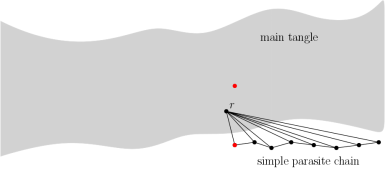
\includegraphics[width=0.45\textwidth]{figures/spc.png}
    \caption{
        An example of simple parasite chain attack, a series of cheat transaction will refer one specific double spent transaction, 
        when the $SPC$ grows to a certain amount, the double spent will be successful, the two red node in the figure respents the 
        conflict transactions.
     }
\label{spc}
\end{center}
\end{figure}

Because the attacker can attack the main network (Main StreamNet) in different forms,
a typical scenario in which we consider the double-spending problem is the Simple Parasite Chain attack.
A simple side chain is shown in Figure~\ref{spc}. 
In \cite{iota_proof}, the author proposed to use local modifier to solve the attack, but since there is no relevant code, we will not discuss it in detail. 
Here we discuss our weight update algorithm with edge information.
The framework of this algorithm is consistent with the framework of the weight update algorithm in the existing DAG.
The difference is that when making a set join between two approve transactions, a weighted set join is performed, and the weight is determined by edges. 
And the information of the edge is mainly determined by time information. 
For example, in Figure~\ref{edge_info}, assume that each edge is assigned a weight $w1$ to $w12$, 
because transaction $5$ is approved by transactions $6$, $7$, $8$, as a result its weight is $[5,7*(w1*w6+*w2) , 8*w3, 6*w6]$.

The reason for the adding of edge information is that the attacker often sends out a large number of transactions 
within a short period of time to achieve the purpose of rapidly growing the side chain. 
If edge information is used to rescale the weight, the effects of these attacks are attenuated. 
On the contrary, becasue the issuing rate of non-attack type transaction is similar to the speed of the whole network,
and its weight update is similar to the result of the original algorithm.

\begin{figure}[!ht]
\begin{center}
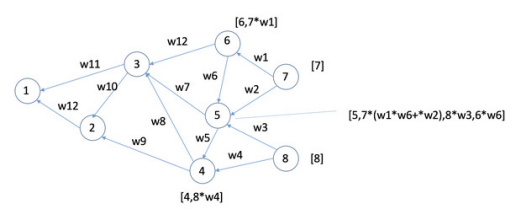
\includegraphics[width=0.55\textwidth]{figures/edge_info.png}
    \caption{
        Weight calculation based on edge information.
     }
\label{edge_info}
\end{center}
\end{figure}

\subsubsection{Weight update algorithm}
When updating the weight, the static graph algorithm needs to recalculate the weight of each node every time when there is an update. 
The complexity of this algorithm is $O(V^2)$. 
If the static result is cached and the new tip is added, by updating the already cached information, the complexity will be amortized. 

